\section{The Language: Trenza}
\label{sec:language}

\subsection{The Minimum Unit: The Context}
\label{sec:context}

The central design decision in Trenza is the identification of the minimum
unit of specification. The answer, borrowed from Reenskaug's DCI
architecture~\cite{reenskaug2009dci}, is the \emph{context}: the smallest
portion of specification that is self-contained and independently verifiable.

A context is not a class. It is not a module. It is the formal description
of a use case---a named situation in which specific roles interact through
specific events to produce specific outcomes. The same data object (a task
card, a navigation tab) can participate in multiple contexts, playing different
roles in each. In \texttt{ModoNormal}, a task card \emph{selects a task} when
tapped. In \texttt{ModoEdicion}, the same card \emph{opens an edit dialog}.
The data is identical; the behavior is contextually determined.

This separation of structure from behavior resolves a problem that
object-oriented programming introduced but never solved: the diamond
inheritance that arises when the same object must behave differently in
different situations. In Trenza there is no inheritance hierarchy. There is a
\texttt{data} layer (what things \emph{are}) and a \texttt{context} layer
(what things \emph{do, here, now}). The two layers never cross.

\subsection{The Four Strands}
\label{sec:strands}

Each Trenza specification generates four artifacts simultaneously---the four
strands of the braid that gives the language its name:

\textbf{Strand~1---Implementation.} A Rust state machine in which each
role-event combination becomes a function with an exhaustive \texttt{match}
over all declared contexts. The choice of Rust is not incidental: Rust's
\texttt{match} enforces the same completeness property as the Trenza verifier,
but at the level of the generated code. The specification is verified by
Trenza; the implementation is verified by \texttt{rustc}. Double verification
from a single source. The same generator pipeline also emits a TypeScript
module for browser environments; TypeScript synthesis is a projection of
Strand~1, not a fifth strand---the four-strand model remains the conceptual
unit.

\textbf{Strand~2---Tests.} The algebraic inverse of the implementation: for
each event-action pair declared in the specification, a test asserts that the
action is produced. The tests are not written; they are derived. If the
specification changes, the tests change. They cannot fall out of sync with the
implementation because they are generated from the same source as the
implementation.

\textbf{Strand~3---Schematics.} A Mermaid statechart diagram of the complete
system topology, including all contexts, transitions, and overlay relationships.
The diagram is always current because it is generated, not drawn.

\textbf{Strand~4---Audit report.} A narrative document that maps each
specification element to a formal verification result, providing the kind of
traceable artifact that GDPR Article~30 and similar regulations require. The
audit cannot be separated from the specification that generated it.

The four strands are projections of a single artifact. Modifying the
\texttt{.trz} regenerates all four. They cannot diverge.

\begin{figure}[h]
  \centering
  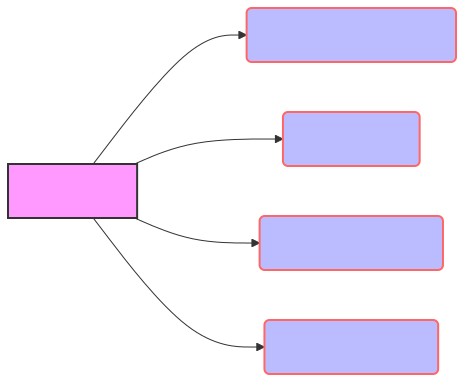
\includegraphics[width=\linewidth]{figures/strands.svg}
  \caption{The four strands of synthesis projected from a single Trenza-DSL specification.}
  \label{fig:strands}
\end{figure}

\subsection{The Eight Rules}
\label{sec:rules}

The behavioral properties that Trenza enforces are expressed as eight
readable rules, checked statically in milliseconds. Each rule closes a
specific class of defect identified in the motivation cases of
Section~\ref{sec:motivation}.

\textbf{Rule~1---Completeness.} Every role that handles an event in any
context must handle that same event in all contexts, even if only with
\texttt{ignored} or \texttt{forbidden}. This rule makes the original
CronometroPSP bug---a handler absent in one context---a compile-time error.
The \texttt{ignored} keyword is not syntactic sugar; it is a declaration of
intent. An absent handler and an \texttt{ignored} handler are structurally
different: the first is an error; the second is a design decision.

\textbf{Rule~2---Determinism.} Each event of each role produces exactly one
action in a given context. No handler may be defined twice. This prevents the
class of defect where two competing handlers produce unpredictable behavior
depending on evaluation order.

\textbf{Rule~3---Reachability.} Every declared context must be reachable from
the initial context through some sequence of transitions. This eliminates dead
specification: contexts that are defined but never activated, which constitute
invisible technical debt.

\textbf{Rule~4---Return.} Every non-initial context must have a path, direct
or indirect, back to the initial context. This prevents sink states---situations
from which the system cannot recover---which are a common failure mode in
manually maintained boolean state.

\textbf{Rule~5---Role exhaustiveness.} Every role declared in the system must
appear in all contexts. If a role exists in one context, its behavior in every
other context must be explicitly accounted for. There is no implicit default.

\textbf{Rule~6---Data conformance.} Data marked with a privacy classification
may only flow to external modules that explicitly declare authorization for
that classification. This rule transforms a class of GDPR compliance
violations---personal data sent to an unauthorized destination by omission or
accident---into a compile-time error. Regulatory compliance becomes structural,
not documentary.

\textbf{Rule~7---Slot/fills integrity.} Concurrent contexts may declare typed
slots that other contexts fill at runtime. Rule~7 verifies, at compile time,
that every declared slot has at least one filling context, that every
\texttt{fills} declaration targets an actual slot, and that the type of the
filling context matches the slot's declared role-set. Without this rule, the
overlay composition primitive---which is what makes complex modal systems like
CronometroPSP expressible---could produce structurally incoherent compositions
that would fail only at runtime.

\textbf{Rule~8---Role-type consistency.} A role name carries a type signature
across the entire specification. If \texttt{EditorTarea} is declared with a
particular event surface in one context, the same name in any other context
must declare the same surface. This prevents a subtle class of defect in which
the same conceptual actor acquires divergent capabilities depending on which
file the reader happens to be looking at---exactly the kind of dispersal that
motivated the language.

Rules~1--5 verify behavioral correctness. Rule~6 verifies regulatory
compliance. Rules~7 and~8 verify compositional and onomastic consistency
across contexts. All eight are first-class citizens in the verifier.

The eight rules are formally equivalent to properties that would be expressed
as temporal logic invariants in TLA+~\cite{lamport2002tla} or as constraints
in Alloy~\cite{jackson2006alloy}. The difference is that a software engineer
can read and discuss them without knowing what a temporal operator is. The
rigor comes from the structure, not the notation.

\subsection{Self-Containment}
\label{sec:selfcontain}

The language is designed so that the specification is the program. There is no
gap between what is declared and what is executed: the \texttt{.trz} file is
the single source of truth from which implementation, tests, schematics, and
audit are derived. The \texttt{.tzp} package format---a signed ZIP containing
all four strands alongside the source specification---embodies this principle:
a single file can be copied, versioned, deployed, and verified without external
dependencies.

This property has a specific consequence for LLM-assisted development. A model
that is given a \texttt{.trz} file has, in a single artefact, both the design
contract and everything needed to verify that any implementation honours it.
There is no separate documentation to consult, no mental reconstruction of
intent from code. The specification is complete and the verification is
mechanical.

\subsection{Multi-Target Synthesis}
\label{sec:multitarget}

The four strands described in Section~\ref{sec:strands} are the conceptual
artifacts every specification produces. Strand~1---the implementation---is
itself parameterized by a target platform. The current compiler emits two
implementation projections from the same \texttt{.trz} source: a Rust state
machine for native and WASM execution, and a TypeScript module for browser
environments. Both projections share the same exhaustiveness guarantees: the
Rust output is verified by \texttt{rustc}'s \texttt{match} exhaustiveness; the
TypeScript output is verified by the compiler itself before emission, since the
TypeScript type system does not enforce exhaustive discriminated-union handling
by default.

Multi-target synthesis is not a generality claim about platforms. It is a
structural claim about the specification: a \texttt{.trz} file describes
behavior at a level of abstraction that admits more than one concrete
realization without recompilation of the source. The same CronometroPSP
specification produces a Rust binary that runs in WASM and a TypeScript module
that runs in a React frontend; both implementations are derived from the same
role-event tables and cannot diverge from each other without diverging from the
source.

This property has direct relevance to the LLM collaboration argument of
Section~\ref{sec:collaboration}. A model asked to make a behavioral change does
not modify two implementations and hope they remain consistent. It modifies the
specification, and the consistency between targets is preserved by construction.
